%%%%%%%%%%%%%%%%%%%%%%%%%%%%%%%%%%%%%%%%%%%%%%%%%%%%%%%%%%%%%%%%%%%%%%%%
% Plantilla TFG/TFM
% Escuela Politécnica Superior de la Universidad de Alicante
% Realizado por: Jose Manuel Requena Plens
% Contacto: info@jmrplens.com / Telegram:@jmrplens
%%%%%%%%%%%%%%%%%%%%%%%%%%%%%%%%%%%%%%%%%%%%%%%%%%%%%%%%%%%%%%%%%%%%%%%%

\chapter{Materials and Methods}
\label{metodologia}
In this section we will go through some of the software and hardware specification related to this work, making special emphasis in those we ended up using as our main resources. We will divide this chapter in 4 different types of resources. First, we needed a game or 3D engine framework in order to generate our synthetic data. Second, we needed a high level deep learning framework in order to implement some of the current architectures, since most of them are quite complex and building them from the ground up is a extremely complex task and out of the scope of this work. Third, we need real world datasets in order to test our synthetic data trained algorithms. And finally, we need extremely powerful GPU computing in order to train and test these architectures.

\section{Unreal Engine 4}
\gls{ue4} is a very powerful, highly portable game engine, written in C++ and developed by Epic Games\footnote{\url{https://www.unrealengine.com/en-US/}}.
The main advantages \gls{ue4} offers over other game engines and the reason UnrealROX was built using it are the following:

\begin{itemize}
	\item \textbf{Virtual reality support:} VR was a key point when developing the ROX framework since one of the main goals was to allow the user to completely interact with the environment.
	\item \textbf{Photorealism:} Realism is a key factor when it comes to synthetic data and \gls{ue4} potential to run extremely realistic scenes, such as the one shown in figure \ref{fig:london_apartment}, in real time made it perfect for this purpose.
	\item \textbf{Blueprints:} Blueprints are one of the tools that \gls{ue4} offers and it allows for quick behavior definitions in the editor without writing a single line of code. This makes it perfect for prototyping and testing.
	\item \textbf{Community:} \gls{ue4} is currently one of the most popular game engines and it has a rather big community, the official forums and other platforms are very active and the official documentation is well maintained. The developing team is very active and they continuously release new versions and bug fixes. 
\end{itemize}

\begin{figure}[h]
	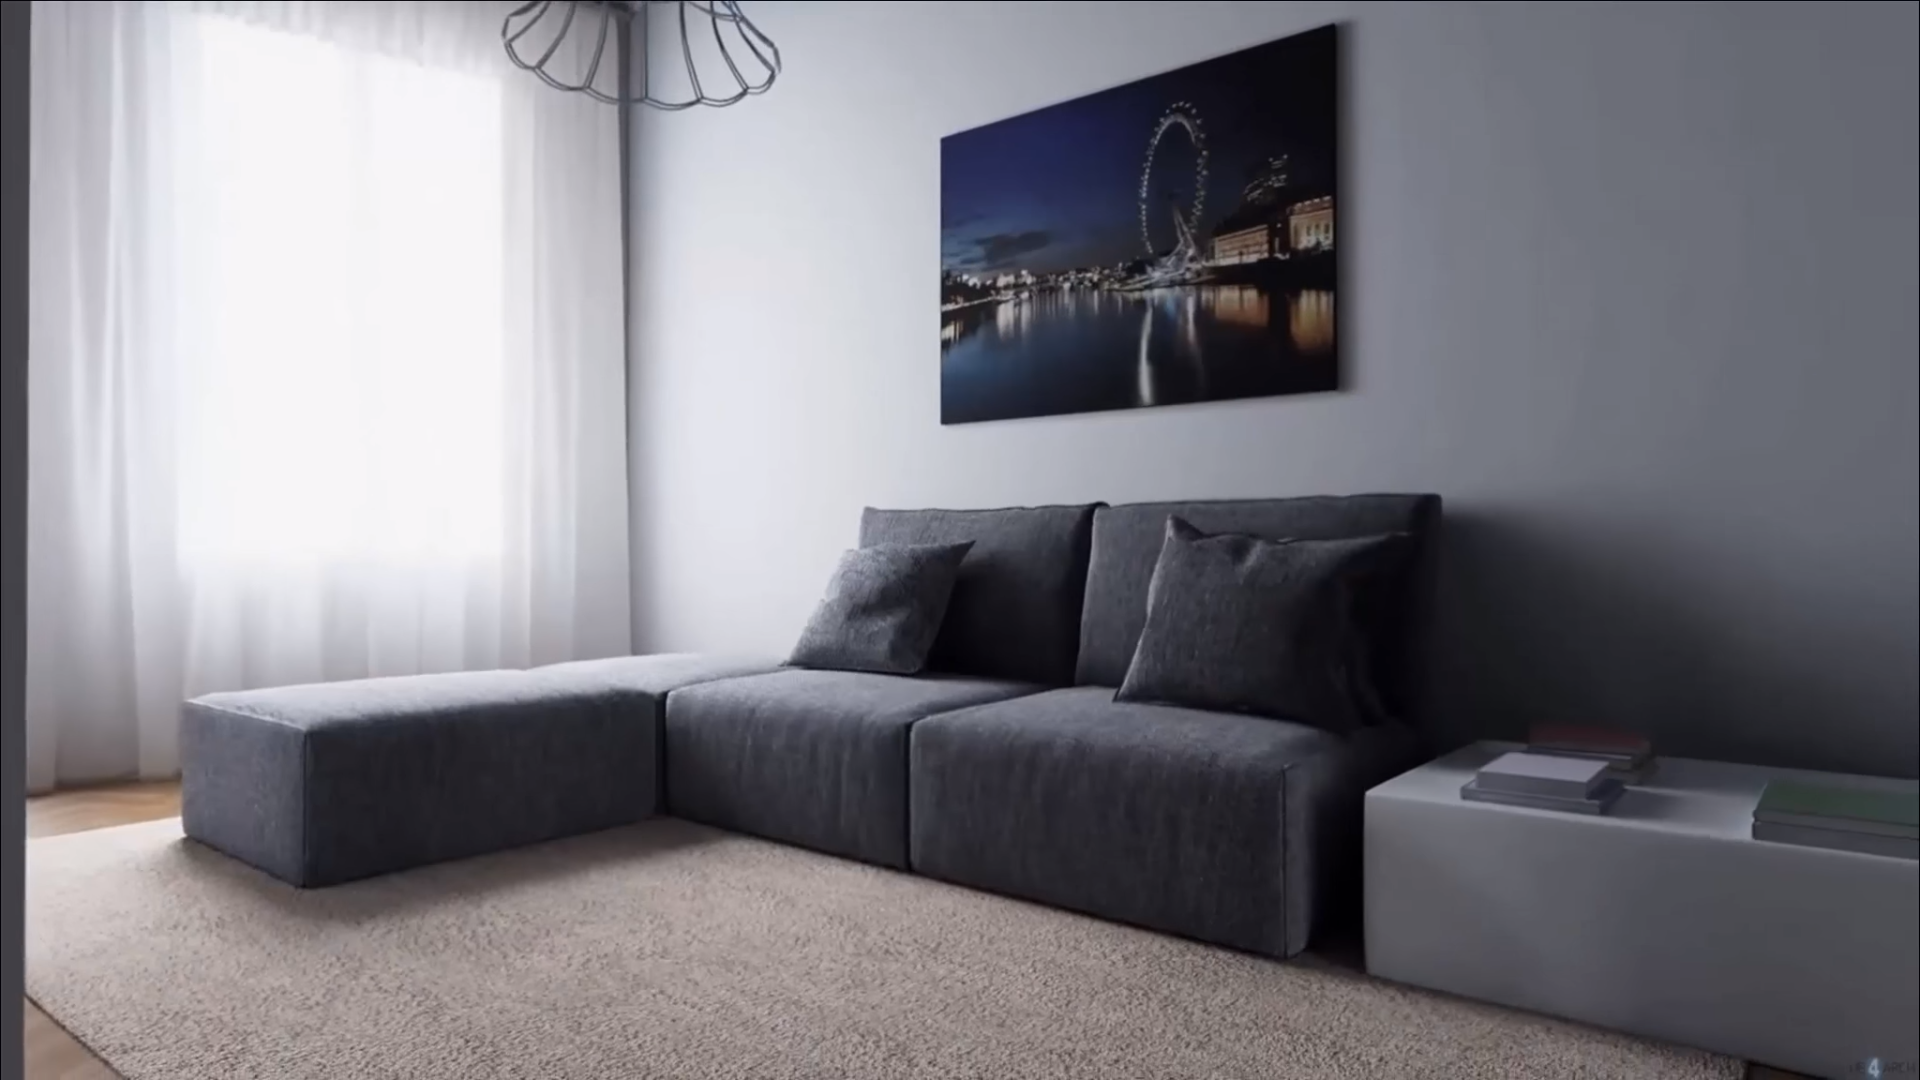
\includegraphics[scale=0.2]{archivos/london_apartment.png}
	\centering
	\caption[Snapshot of the Viennese Apartbent by UE4Arch]{Snapshot of the Viennese Apartment by UE4Arch\footnotemark}
	\label{fig:london_apartment}
\end{figure}
\footnotetext{\url{https://ue4arch.com/projects/viennese-apartment/}}



\section{Frameworks}

In this section, we will go trough some of the most recent and popular \gls{dl} frameworks.

\subsection{TensorFlow}
TensorFlow is a open source library for numerical computation based on the idea of data flow graphs. In TensorFlow, the graph nodes represent the mathematical operations, while the edges represent the multidimensional data arrays (or tensors) flowing between them.

TensorFlow was created by the researches at Google Brain for the purpose of conducting machine learning and deep neural network research, its low level nature allows for a very fine-grained framework that can be use to build any architecture from the ground up and the tensor-graph structure also allows for very easy distribution on the CPU-GPU.

\todo{add flow graph figure}

In a first approach, TensorFlow was going to be the main framework for this project, but was finally discarded since high level frameworks will ease the work and the low level implementation of the networks fall out of the scope of this project.

\subsection{Keras}
Keras is a high level framework written in Java that can use TensorFlow, CNTK or Theano as backend. It was developed with a focus on allowing for very fast experimentation and prototyping, abstracting the user of some of the more complex low level tasks with a very user friendly interface. This also makes Keras a very good entry framework for beginners that still don't have a solid foundation on deep learning.

Keras provides two different API's for different model building approaches. The Sequential API which allows to simply stack layer after layer, allowing for a very simple and easy to use interface for models with a input to output data flow. The Functional API however allows for more complex models by understanding each layer as a node graph, allowing for different, more complex and non sequential models.
 
\subsection{PyTorch}
PyTorch is an open source, Python-based computing package and machine learning framework.

PyTorch was the framework of choice for this project since it allows for easy prototyping without losing the flexibility make architectural modifications to the networks. Its syntax is also very easy for anyone that has experience with python which made it perfect for this project.

\subsection{UnrealROX}
 